\chapter{In-Hand Manipulation}\label{ch:3-in-hand-manipulation}

The goal of this chapter is to analyze the performance of the \gls{rl}-based manipulation algorithm \gls{dapg}, which employs \gls{il} to constrain the algorithm's search space when solving the relocation task, as well as compare the final performance with the \gls{dapg} algorithm trained by the authors of~\cite{dexmv:-imitation-learning-for-dexterous-manipulation-from-human-videos}. The relocation task requires the robot hand to pick up an object and move it to a target location.\medskip 

The analysis will focus on the relevant metrics from the training process as well as the final model's performance. \gls{dapg} was chosen as the algorithm from~\cite{dexmv:-imitation-learning-for-dexterous-manipulation-from-human-videos}, due to it showing the best performance when solving the relocation task. \medskip

The structure of this chapter follows a logical progression. It begins with the presentation of the problem formulation, providing context regarding the problem structure and mathematical expressions formulations. Next, the \gls{dapg} method is introduced and described in detail, outlining its key components and principles. Following that, the experimental setup for data collection, which is used for training the algorithm, is presented.\medskip

Once the data is collected and the algorithm is trained, the results obtained are presented and analyzed. This analysis includes evaluating the success of training the model as well as comparing the performance of the \gls{dapg} method in addressing the problem, with the performance of the model trained by the authors. The findings from the analysis are then discussed, providing insights and interpretations of the results. \medskip

Finally, the chapter concludes by summarizing the main points, discussing the implications of the findings, and highlighting potential future directions.\medskip

% This chapter is structured such that, the problem formulation is presented first, followed by the \gls{dapg} method being presented and described. Aftwewhich the experimental setup for collecting the data used for training. The results are then presented and analyzed, finally, the findings are discussed and concluded.\medskip

The simulation is done using a \gls{ah}~\cite{learning-complex-dexterous-manipulation-with-deep-reinforcement-learning-and-demonstrations} in the dynamic simulator MuJoCo~\cite{todorov2012mujoco}. The hand is thus equipped with \num{30} controllable parameters, \num{24} for the hand's joints and \num{6} for the hand's position \mvar{\vec{p}_{hnd}=\rvec{p_x,p_y,p_z}} and orientation \mvar{\vec{u}=\rvec{\phi,\theta,\psi}} in \gls{rpy} format. These make up the agent's actions \mvar{a}, while the states {s} also include the position of the prop when performing the relocation task.

\section{Problem Formulation}\label{sec:3-in-hand-manipulation-problem-formulation}

\gls{rl} aims to solve a control problem in the form of a \gls{mdp}, denoted by \mvar{\mathcal{M} = \{\mathcal{S}, \mathcal{A}, \mathcal{R}, \mathcal{T}, \rho_0, \gamma\}}. The \gls{mdp} consists of a state space \mvar{\mathcal{S} \inR{n}}, an action space \mvar{\mathcal{A} \inR{m}}, a reward function \mvar{\mathcal{R}(s, a): \mathcal{S} \times \mathcal{A} \rightarrow \mathcal{R}}, transition dynamics \mvar{\mathcal{T}(s, a): \mathcal{S} \times \mathcal{A} \rightarrow \mathcal{S}}, an initial state distribution \mvar{\rho_0}, and a discount factor \mvar{\gamma \in [0, 1]} that determines the importance of future rewards. \medskip

The objective in \gls{rl} is to find a stochastic policy \mvar{\pi: \mathcal{S} \times \mathcal{A} \rightarrow \mathcal{R}_+} that maximizes the expected sum of rewards
%
\begin{equation}
	\eta(\pi) = \mathbb{E}_{\pi, \mathcal{M}} \left[\sum_t \gamma^t r_t\right],
\end{equation}
where \mvar{\mathbb{E}_{\pi, \mathcal{M}}} denotes the expectation with respect to the policy \mvar{\pi} and the \gls{mdp} \mvar{\mathcal{M}}. The policy parameters \mvar{\theta} are updated to optimize this expected sum of rewards.\medskip

In practice, learning \gls{rl} policies from scratch can be challenging and sample-intensive. However, by incorporating a set of demonstration data denoted as \mvar{\rho_D}, which contains state-action-state-reward tuples \mvar{(s_t, a_t, s_{t+1}, r_t)}, the sample complexity of \gls{rl} can significantly be reduced. These demonstrations provide valuable guidance and can be used to improve the learning process.

\section{Method}\label{sec:3-in-hand-manipulation-method}

\subsection{Demo Augmented Policy Gradient}\label{dapg}

The \gls{dapg} algorithm addresses the \gls{rl} problem by combining the principles of \gls{npg}s and the use of demonstration data. It consists of two main components: pretraining with \gls{bc} and \gls{rl} fine-tuning with augmented loss. \medskip

The pretraining with \gls{bc} works by enhancing the exploration and providing an informed policy initialization. \gls{bc} aims to mimic the actions taken in the demonstrations by solving a maximum-likelihood problem. The objective is to maximize the log probability of actions given states
%
\begin{equation}
	\max_{\theta} \sum_{(s, a) \in \rho_D} \log \pi_{\theta}(a|s).
\end{equation}

\gls{bc} can efficiently guide exploration, reducing the reliance on reward-shaping techniques commonly used to direct exploration in \gls{rl}. \medskip

The process of \gls{rl} fine-tuning with augmented loss involves effectively utilizing the comprehensive information provided by the demonstrations. Although \gls{bc} serves as a suitable initialization, it doesn't fully utilize the full information contained within the demonstration data. Notably, different segments of the demonstration data hold value during various stages of learning, especially in tasks that require sequential behaviors. To leverage the complete range of information embedded in the demonstrations, an augmented loss is introduced.\medskip

% The \gls{rl} fine-tuning with augmented loss works by extracting complete information from the demonstration. While \gls{bc} provides a good initialization, it does not fully exploit the information in the demonstration data. Different parts of the demonstration data are useful at different stages of learning, particularly for tasks involving sequential behaviors. To leverage the complete information from the demonstrations, an augmented loss is introduced.\medskip

The augmented gradient \mvar{g_{aug}} is defined as the sum of two terms
%
\begin{equation} \label{eq:dapg-grad}
	g_{aug} = \sum_{(s,a)\in\rho_{\pi_\theta}}\nabla_\theta \ln \pi_\theta(a|s)A^{\pi_\theta}(s,a) + \sum_{(s,a)\in\rho_{\pi_D}} \nabla_\theta \ln \pi_\theta(a|s) w(s,a).
\end{equation}

The first term considers state-action pairs \mvar{(s, a)} sampled from the occupancy measure \mvar{\rho_{\pi}}, which represents the probability of encountering a specific state-action tuple. This term is weighted by the advantage function \mvar{A^{\pi}(s, a)}, which quantifies the advantage gained by taking action \mvar{a} in state \mvar{s} compared to the expected return from the currently best action. Additionally, the \mvar{\nabla_\theta} is the gradient with regards to \mvar{\theta}.\medskip

The second term in \mvar{g_{aug}} sums over the state-action pairs \mvar{(s, a)} from the demonstrations dataset \mvar{\rho_D}. The gradient of the logarithm of the policy \mvar{\pi_{\theta}(a|s)} is multiplied by a weighting function \mvar{w(s, a)}. This term allows the algorithm to leverage the knowledge provided by the demonstrations to guide the learning process. \medskip

The \gls{dapg} algorithm updates the policy parameters \mvar{\theta} using the \gls{npg} and the demonstration-augmented gradient. The parameter update rule involves the \gls{fim} and the gradient, as shown in the update rule
%
\begin{equation}
	\theta_{k+1} = \theta_k + \sqrt{\frac{\delta}{g^\T F^{-1}_{\theta_k}g}}F^{-1}_{\theta_k}g,
\end{equation}

where \mvar{\delta} is the step size that determines the magnitude of the update. \medskip

The choice of the weighting function \mvar{w(s, a)} in~\eqref{eq:dapg-grad} is critical. While an ideal choice would be \mvar{w(s, a) = A^{\pi}(s, a)} for \mvar{(s, a) \in \rho_D}, computing this quantity exactly requires additional rollouts or assumptions. Therefore, a heuristic weighting scheme is typically used. For example, 
%
\begin{equation}
	w(s, a) = \lambda_0 \lambda_1^k \max_{(s_0, a_0) \in \rho_{\pi}} A^{\pi}(s_0, a_0)
\end{equation}
can be used, where \mvar{\lambda_0} and \mvar{\lambda_1} are hyperparameters, and \mvar{k} is the iteration counter. The decay of the weighting term via \mvar{\lambda_1^k} ensures that the guidance from demonstrations gradually diminishes as the policy's performance improves. \medskip

In summary, the \gls{dapg} algorithm combines \gls{bc} with \gls{rl} to effectively learn complex behaviors. By utilizing the demonstrations for policy initialization and then fine-tuning the policy using both imitation and reinforcement learning, \gls{dapg} benefits from the strengths of both approaches. This combination allows for more efficient and effective learning, reducing the sample complexity and accelerating the convergence of \gls{rl} algorithms.





% The goal is to determine a stochastic policy on the form \mvar{\pi: s\times a \rightarrow \R_+}, which optimizes the expected sum of rewards
% %
% \begin{equation}
% 	\eta(\pi)=\mathbb{E}_{\pi,\mathcal{M}} \left[ \sum^\infty_{t=0} \gamma^t r_t \right]
% \end{equation}
% where \mvar{\mathcal{M}=\{ \mathcal{S},\mathcal{A},\mathcal{R},\mathcal{T},\rho_0,\gamma \}} is a \gls{mdp} consisting of states \mvar{\mathcal{S}\inR{n}}, actions \mvar{\mathcal{A}\inR{m}}, rewards \mvar{\mathcal{R}}, transition dynamics \mvar{\mathcal{T}}, \mvar{\rho_0} the probability distribution over initial states and \mvar{\gamma\in[0,1]} being the discount factor.\medskip

% Additionally, the value, \mvar{Q} and advantage functions are needed i.e.
% \begin{equation}
% 	V^\pi(s)=\mathbb{E}_{\pi,\mathbb{M}}\left[ \sum^\infty_{t=0} \gamma^t r_t | s_0 = s \right]
% \end{equation}
% \begin{equation}
% 	Q^\pi(s,a)=\mathbb{E}_{\mathbb{M}}\left[ \mathbb{R}(s,a) \right] + \mathbb{E}_{s'\sim \mathbb{T}(s,a)\left[ V^\pi (s') \right]}
% \end{equation}
% \begin{equation}
% 	A^\pi(s,a) = Q^\pi (s,a) - V^\pi (s)
% \end{equation}
% To optimize wrt. \mvar{\pi_\theta} the optimization is done wrt. parameters \mvar{\theta}.

% The \gls{dapg} is an approach that expands on the \gls{npg} by introducing a demonstration term to weigh the gradient by \mvar{\lambda_0} and \mvar{\lambda_1}, which are hyperparameters to determine the advantage of state-action pair in demonstrations. \medskip

% The parameter update rule to gain \mvar{\theta_{k+1}} can be written as
% %
% \begin{equation}
%     \theta_{k+1} = \theta_k + \sqrt{\frac{\delta}{g^\T F^{-1}_{\theta_k}g}}F^{-1}_{\theta_k}g,
% \end{equation}
% where \mvar{F_{\theta_k}} is the \gls{fim}, \mvar{g} is the gradient, \mvar{\delta} is the step size, and \mvar{\theta_{k}} is the previous weights.\medskip

% The objective function is thus formulated as 
% %
% \begin{equation}\label{eq:dapg}
%     g_{aug} = \sum_{(s,a)\in\rho_{\pi_\theta}}\nabla_\theta \ln \pi_\theta(a|s)A^{\pi_\theta}(s,a) + \sum_{(s,a)\in\rho_{\pi_D}} \nabla_\theta \ln \pi_\theta(a|s) \lambda_0 \lambda_1^k
% \end{equation}

% Here \mvar{\rho_{\pi_\theta}} is the occupancy measure, which is the probability of ending up in a state action tuple i.e. \mvar{(s,a)}, \mvar{\nabla_\theta} is the derivative operator in terms of \mvar{\theta}, \mvar{\pi_\theta} is the policy under the parameters \mvar{\theta}, \mvar{A^{\pi_\theta}} is the advantage function which tells the advantage gained by performing each action \mvar{\{a_1,a_2,\dots,a_{n_a}\}}, where \mvar{n_a} is the number of actions in the current state, compared to the expected return from taking the currently best action~\cite{advantage-updating}. Finally, \mvar{\rho_{\pi_D}} is the occupancy function from the demonstrations.

\subsection{Data Collection Procedure}
To train \gls{dapg}, raw video data of expert demonstrations of the relocation task is collected. While~\cite{dexmv:-imitation-learning-for-dexterous-manipulation-from-human-videos} provides data for additional tasks i.e. \textit{pour} and \textit{place inside}, these are not of interest in this chapter. The objects used are from the YCB dataset~\cite{ycb} and the demonstrations were recorded by two RGBD cameras.\medskip

The collected data are then parsed to a multi-state pipeline including 3D \gls{pe}, for estimating the pose of both the object of interest and the hand for demonstration translation.

\subsubsection{Object Pose Estimation}
The \num{6}-\gls{dof} object poses in the physical setup is found using the PVN3D model, which is a \gls{dl}-based \gls{pe} model, trained on the YCB data set.\medskip

The \num{6}-\gls{dof} object pose is afterward optimized by minimizing the \gls{PnP} matching error.

\subsubsection{Hand Pose Estimation}

The hand pose is found using the \gls{dl}-based \gls{pe} model MANO~\cite{mano}, which produces three parameters to represent the hand's pose: \mvar{\theta_t},\mvar{\beta_t} and \mvar{r_t}. \mvar{\theta_t} refers to the 3D rotations of \num{15} joints, \mvar{\beta_t} is the shape parameters and \mvar{r_t} is the hand root's global pose~\cite{mano}. These can be combined through hand kinematics to compute the 3D angle of each hand joint
%
\begin{equation}
    \vec{q}^{3d}_t = \mat{J}(\theta_t,\beta_t,r_t)
\end{equation}

By utilizing off-the-shelf skin segmentation techniques such as Combinatorial Color Space Models~\cite{combinatorial-color-space-models-for-skin-detection-in-sub-continental-human-images} and hand detection models on video data, a hand mask \mvar{M_t} is extracted. \mvar{M_t} is overlayed the depth channel of the recorded data, the center of which is the used estimate of \mvar{r_t}. From the video data, the RGB channels are additionally parsed to a MANO which estimates 2D hand joint angles \mvar{\vec{q}_t^{2D}}, along with the hand parameters \mvar{(\theta_t,\beta_t,r_t)}. Having the cameras poses \mat{\Pi} enables the formulation of an optimization problem to determine the optimal \mvar{(\theta_t,\beta_t,r_t)} i.e. \mvar{(\theta_t^\star,\beta_t^\star,r_t^\star)}
%
\begin{equation}
    \theta_t^\star,\beta_t^\star, r_t^\star = \argmin_{\theta_t,\beta_t,r_t} \| \mat{\Pi} \mat{J}(\theta_t,\beta_t, r_t) - \vec{q}_t^{2d} \|^2 + \lambda\| M_t \left( \mat{R}(\theta_t,\beta_t,r_t) - D_t \right) \|^2.
\end{equation}
Here \mvar{\lambda=0.001} is a hyperparameter, \mat{R} is a depth rendering function and \mvar{D_t} is the corresponding depth map in frame \mvar{t}.

\subsubsection{Demonstration Translation}

Demonstration translation involves transforming the actions performed by the expert agent, with one kinematic structure, to a \gls{ml} agent with some other set of actions. This is essential as, while the kinematic structure between the biological human hand and the anthropomorphic robot hand is similar, they are not identical. The similarity can be seen in the hands' kinematic trees in~\appref{app:human-and-robot-hand-kinematics} with their \gls{rom}s in~\appref{app:range-of-motion-shadow-hand} and~\appref{app:range-of-motion-human-hand}.\medskip

Demonstration translation requires two components: hand motion retargeting and Predicting robot action. The hand motion retargeting attempts to align the human hand motion to the robot hand motion, which due to the difference in kinematics is non-trivial as mentioned above. The prediction of robot actions attempts to estimate the torque necessary for each robot motor to recover the action from only \gls{pe} results. \medskip

The hand motion retargeting is solved using \gls{tsv}s to describe the optimization problem
%
\begin{equation}
    \vec{q}^\star_t = \min_{\vec{q}_t} \sum^N_{i=1}\| \vec{v}^{hum}_i(\theta_t,\beta_t,r_t)-\vec{v}^{rob}_i(\vec{q}_t)\|^2+\alpha \| \vec{q}_t - \vec{q}_{t-1} \|^2.
\end{equation}
Here \mvar{\vec{v}^{hum}_i(\theta_t,\beta_t,r_t)} computes the \mvar{i}'th \gls{tsv} to the fingertip and finger middle joint of the human hand, while the robot's forward kinematics function \mvar{\vec{v}^{rob}_i(\vec{q})} computes the \mvar{i}'th \gls{tsv} to the fingertip and finger middle joint of the robot hand. The \gls{tsv}s can be seen illustrated in~\figref{fig:tsv} from the hand root (marked with red) to the finger middle joint (marked with blue) and tip (marked with green) on the anthropomorphic robot hand.\medskip

\begin{figure}[!h]
	\begin{center}
		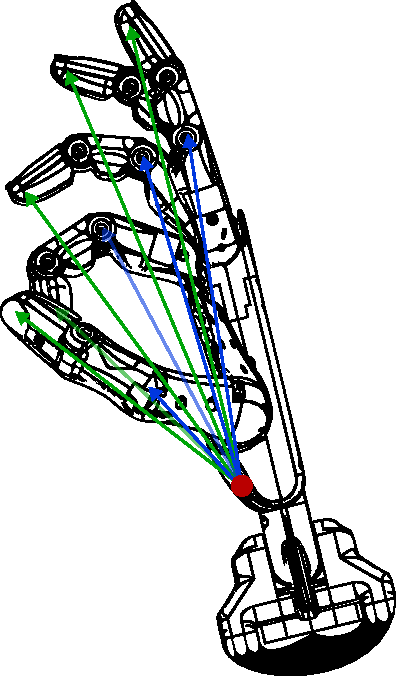
\includegraphics[width=0.3\textwidth]{chapters/3-in-hand-manipulation/fig/tsv.pdf}
	\end{center}
	\caption{The \gls{tsv}s from the hand root (marked with red) to the finger middle joint (marked with blue) and tip (marked with green) on the anthropomorphic robot hand.}
	\label{fig:tsv}
\end{figure}

The optimization problem was solved using \gls{slsqp} with \mvar{\alpha = 8e-3}.\medskip

The robot action estimation is achieved through the model \mvar{\vec{q}(t)} presented in~\cite{smoothness-maximization-along-a-predefined-path-accurately-predicts-the-speed-profiles-of-complex-arm-movements}, which fulfills the criteria of approximately zero jerk i.e. \mvar{\vec{q}'''(t) \approx 0}. The model enables \mvar{\vec{q}'(t)} and \mvar{\vec{q}''(t)} which through inverse dynamics can be converted to toques \mvar{\vec{\tau}}
%
\begin{equation}
    \vec{\tau} = f_{inv}\left(\vec{q}(t),\vec{q}'(t),\vec{q}''(t)\right)
\end{equation}
The zero jerk here enables behavior similar to that of a human, which in turn leads to more natural robot motion, as well as ensuring low joint position errors for motors and limiting excessive wear on the physical robot.

\section{Experimental Setup}\label{sec:3-in-hand-manipulation-experimental-setup}

To train and test the \gls{dapg} algorithm, the mug shown in~\figref{fig:manipulation-mug} is chosen as the prop from YCB. Additionally, to remain consistent with the original paper~\cite{dexmv:-imitation-learning-for-dexterous-manipulation-from-human-videos} the number of training iterations was set to \num{2000} with demonstration hyperparameters \mvar{\lambda_0} and \mvar{\lambda_1} being \num{0.1} and \num{0.99} respectively. Furthermore, the learning rate \mvar{\alpha_{lr}} was set to \num{1.0}, the step size \mvar{\delta} was set to \mvar{0.1} and the discount factor \mvar{\gamma} was set to \num{0.995}. This however will result in the same performance, and thus to test the consistency of \gls{dapg}, a different seed is used for randomization. The seed used in the authors' paper~\cite{dexmv:-imitation-learning-for-dexterous-manipulation-from-human-videos} is \num{200}, while the one chosen for this project is \num{201}. \medskip

To execute the relocation task, the object is placed on a table and a goal is defined at a random location marked with green silhouette. The experimental setup can be seen in~\figref{fig:experimental-setup-dapg}.

% \begin{figure}[!h]
% 	\centering
% 	\begin{subfigure}[b]{0.48\textwidth}
% 		\centering
% 		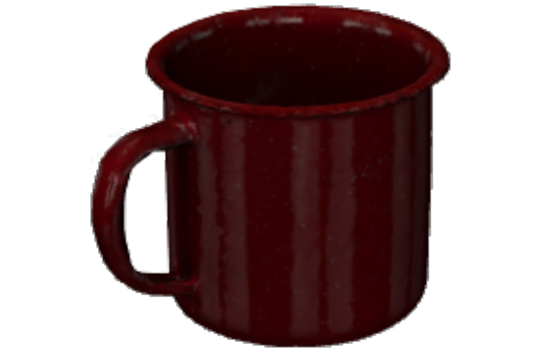
\includegraphics[width=\textwidth]{chapters/3-in-hand-manipulation/fig/mug.pdf}
% 		\caption{The mug prop from YCB~\cite{ycb} chosen for training.}
% 		\label{fig:manipulation-mug}
% 	\end{subfigure}
% 	\hfill
% 	\begin{subfigure}[b]{0.48\textwidth}
% 		\centering
% 		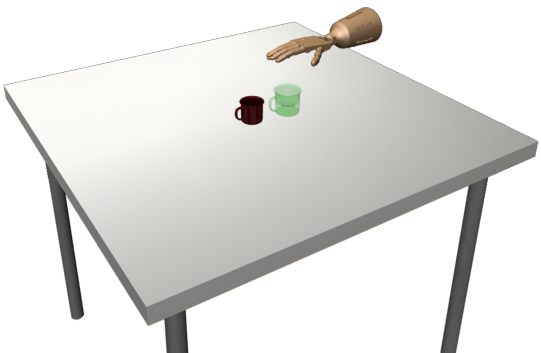
\includegraphics[width=\textwidth]{chapters/3-in-hand-manipulation/fig/experimental-setup-dapg.pdf}
% 		\caption{The experimental setup used when training the \gls{dapg} algorithm. The figure contains the table platform, the mug prop, the simulated anthropomorphic hand and the goal mug position marked as a green silhouette.}
% 		\label{fig:experimental-setup-dapg}
% 	\end{subfigure}
% 	\caption{The mug prop used for training and the experimental setup.}
% 	\label{fig:manipulation-mug-experimental-setup-dapg}
% \end{figure}


\begin{center}
    \renewcommand{\arraystretch}{1.2}
    \begin{minipage}{.48\linewidth}
        \vspace{0pt}
        \centering
        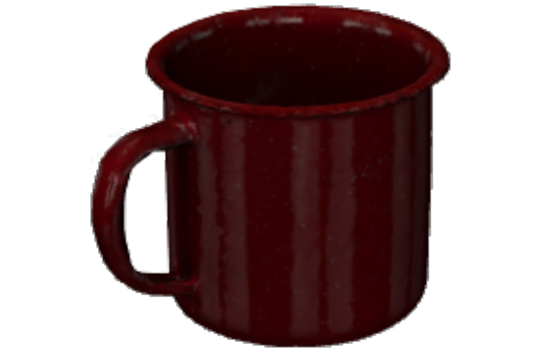
\includegraphics[width=.95\textwidth]{chapters/3-in-hand-manipulation/fig/mug.pdf}
    \end{minipage}%
    \hfill%
    \begin{minipage}{.48\linewidth}
        \vspace{0pt}
        \centering
        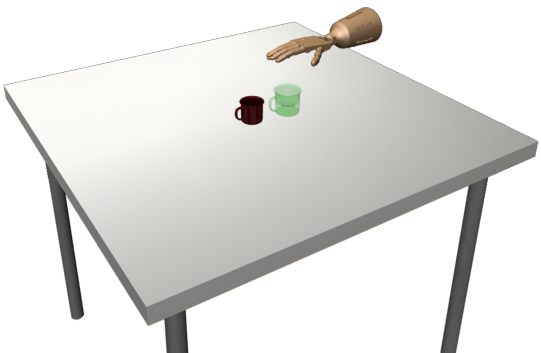
\includegraphics[width=.95\textwidth]{chapters/3-in-hand-manipulation/fig/experimental-setup-dapg.pdf}
    \end{minipage}%
    %    
    \vspace{15pt}
    %
    \begin{minipage}[t]{.4\linewidth}
        \vspace{0pt}
        \captionsetup{type=table}
        \captionof{table}{The mug prop from YCB~\cite{ycb} chosen for training.}
        \label{fig:manipulation-mug}
    \end{minipage}%
    \hfill%
    \begin{minipage}[t]{.55\linewidth}
        \vspace{0pt}
        \captionsetup{type=figure}
        \captionof{figure}{The experimental setup used when training the \gls{dapg} algorithm. The figure contains the table platform, the mug prop, the simulated anthropomorphic hand and the goal mug position marked as a green silhouette.}
        \label{fig:experimental-setup-dapg}
    \end{minipage}%
\end{center}



\section{Results}\label{3-in-hand-manipulation-results}

The evaluation score of the \gls{rl} agent on a separate set of test episodes can be seen in~\figref{fig:evaluation-score-over-epochs}, the running score obtained by the \gls{rl} agent during training can be seen in~\figref{fig:running-score-over-epochs}, and finally, the expected return used in policy i.e. the improvement or increase in the surrogate objective function during the policy update can be seen in figure~\figref{fig:surrogate-improvements-over-epochs}.

\begin{figure}[!h]
	\begin{center}
		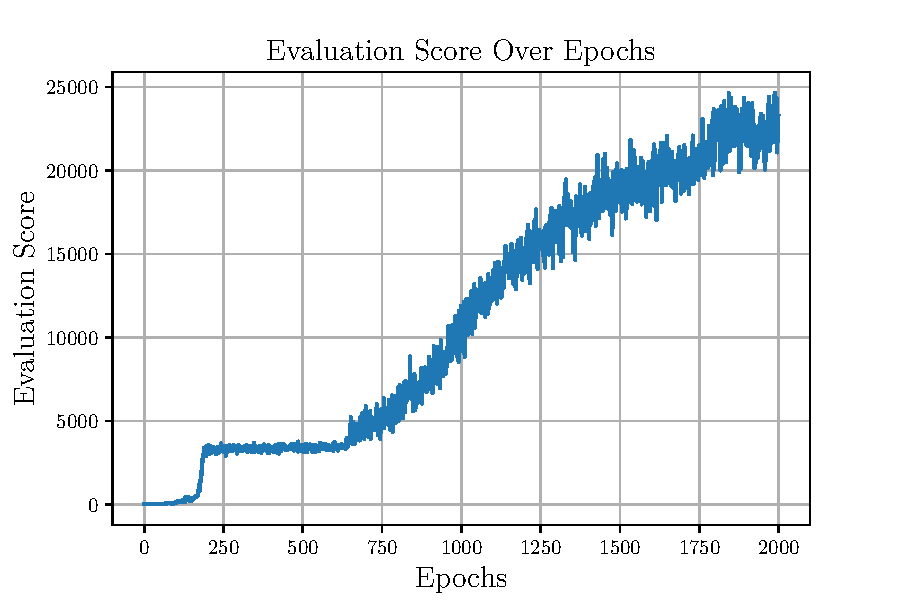
\includegraphics[width=0.8\textwidth]{chapters/3-in-hand-manipulation/fig/evaluation-score-over-epochs.pdf}
	\end{center}
	\caption{The evaluation score of the \gls{dapg} agent on a separate set of test episodes or environments.}
	\label{fig:evaluation-score-over-epochs}
\end{figure}

\begin{figure}[!h]
	\begin{center}
		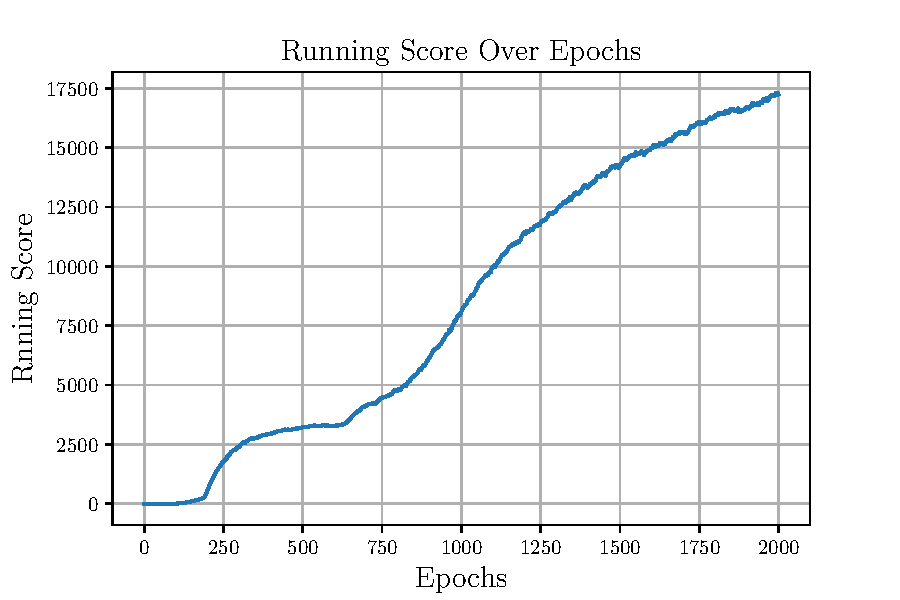
\includegraphics[width=0.8\textwidth]{chapters/3-in-hand-manipulation/fig/running-score-over-epochs.pdf}
	\end{center}
	\caption{The running score shows the cumulative reward obtained by the \gls{dapg} agent during training.}
	\label{fig:running-score-over-epochs}
\end{figure}

\begin{figure}[!h]
	\begin{center}
		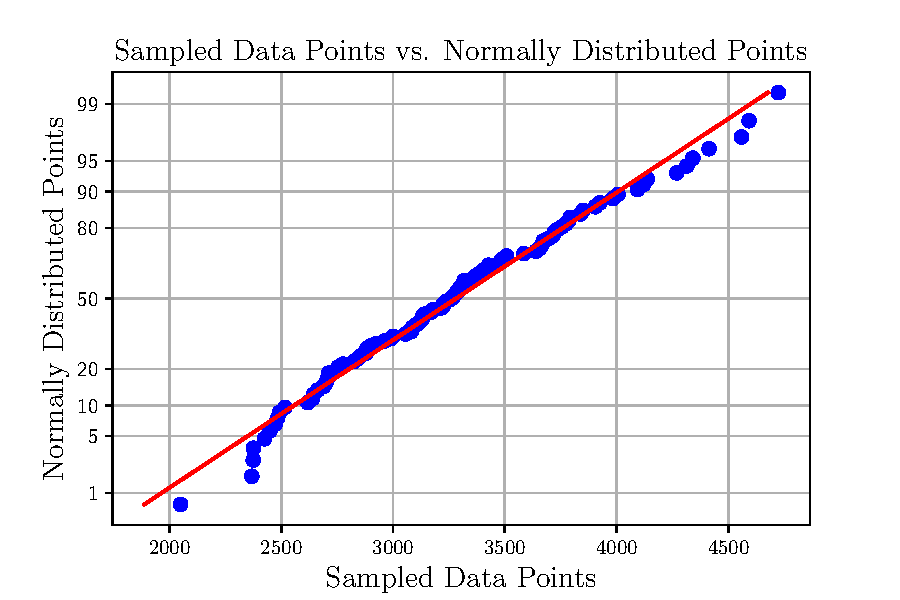
\includegraphics[width=0.8\textwidth]{chapters/3-in-hand-manipulation/fig/surrogate-improvements-over-epochs.pdf}
	\end{center}
	\caption{The increase in the surrogate objective function during the policy update.}
	\label{fig:surrogate-improvements-over-epochs}
\end{figure}
\newpage
Once trained, the best policy was saved and the reward was sampled over \num{100} iterations, both for the model trained and the one provided by the authors resulting in~\figref{fig:probability-of-getting-a-reward}, showing the probability distributions for each algorithm's best policy rewards.
\newpage
\begin{figure}[!h]
	\begin{center}
		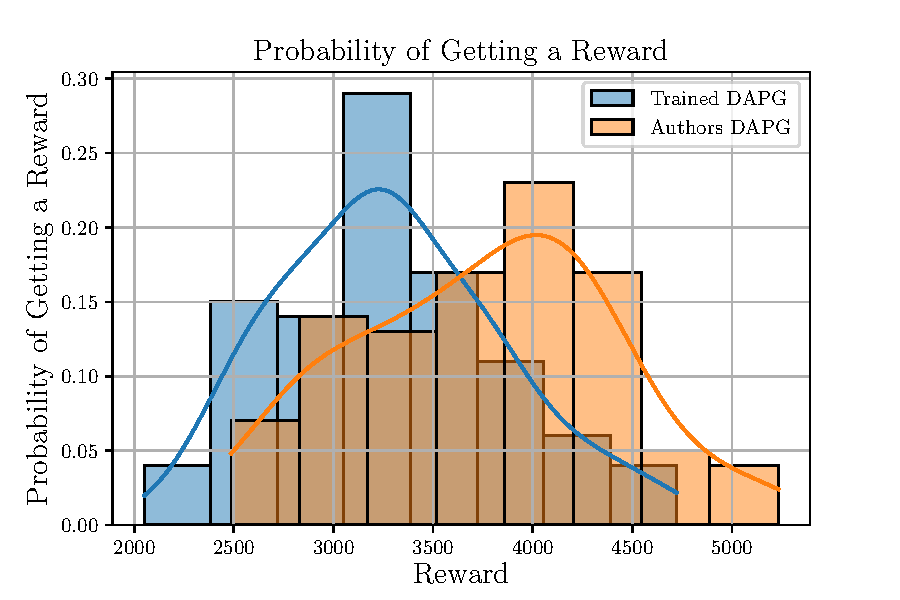
\includegraphics[width=0.8\textwidth]{chapters/3-in-hand-manipulation/fig/probability-of-getting-a-reward.pdf}
	\end{center}
	\caption{Histograms showing the probability distributions of getting certain rewards over \num{100} iterations for both the authors' and the trained \gls{dapg} algorithms.}
	\label{fig:probability-of-getting-a-reward}
\end{figure}

The mean of each distribution is found to be \mvar{\mu_{trained}\approx 3276.1} and \mvar{\mu_{authors}\approx 3759.4}. \medskip

\figref{fig:ai-frames} show the three stages throughout the \gls{pnp} process of the relocation phase as executed when the distributions were sampled.

\begin{figure}[!h]
	\centering
	\begin{subfigure}[b]{0.32\textwidth}
		\centering
		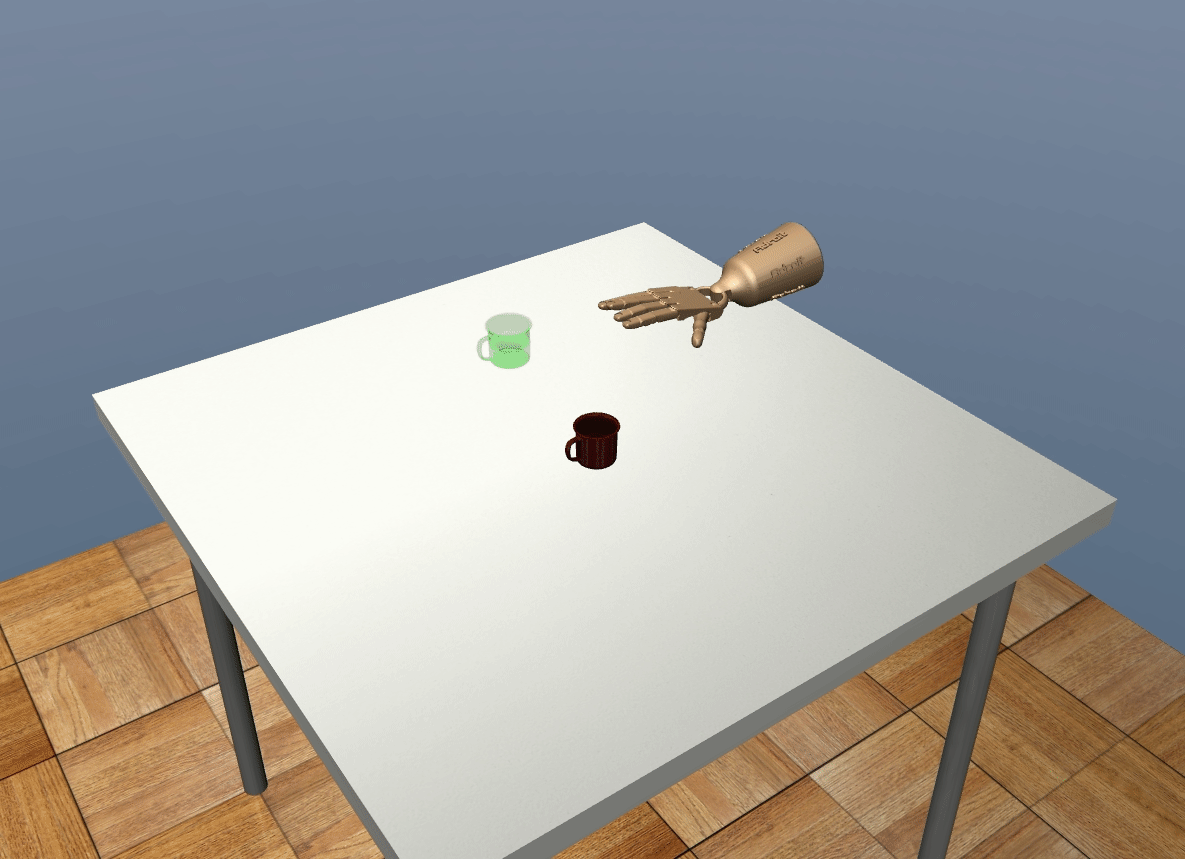
\includegraphics[width=\textwidth]{chapters/3-in-hand-manipulation/fig/frame_10.png}
		\caption{The pre-grasping phase, where the \gls{ah} is moving towards the mug.}
		\label{fig:ai-frame-1}
	\end{subfigure}
	\hfill
	\begin{subfigure}[b]{0.32\textwidth}
		\centering
		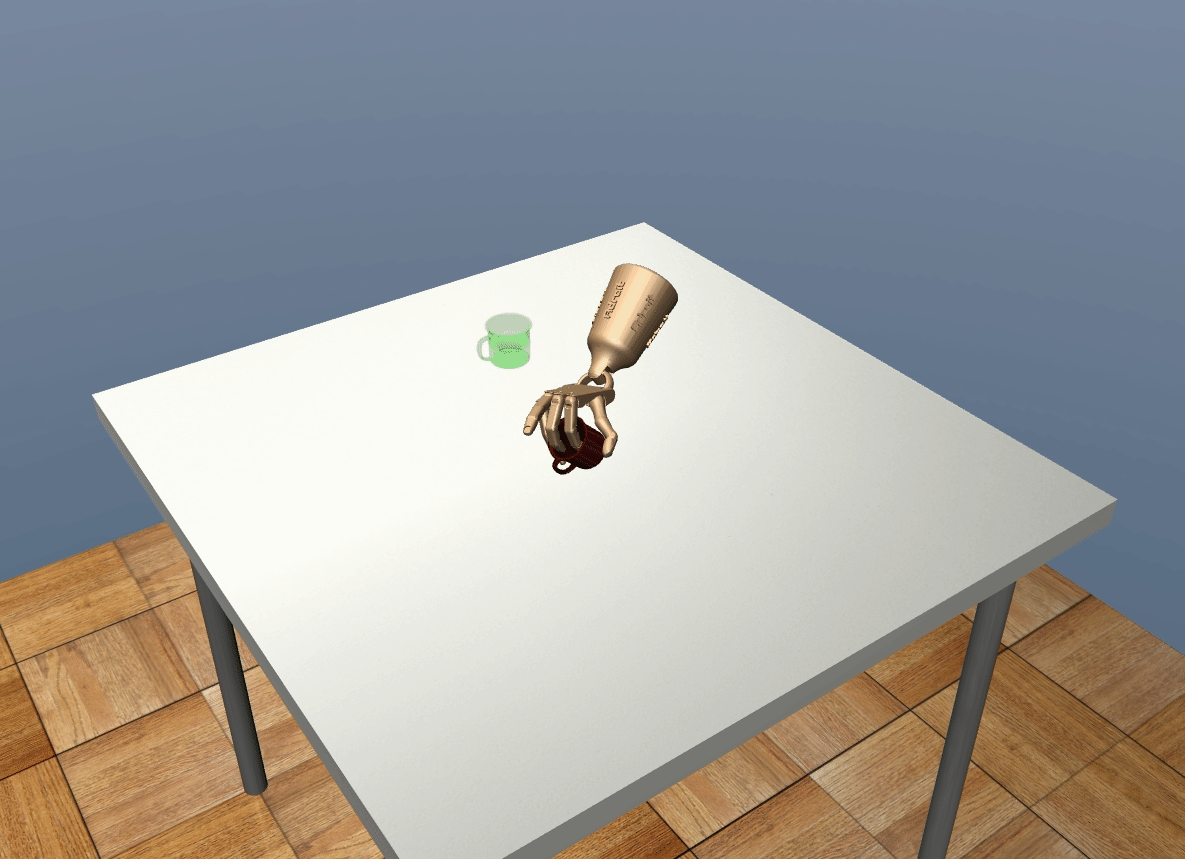
\includegraphics[width=\textwidth]{chapters/3-in-hand-manipulation/fig/frame_21.png}
		\caption{The grasping phase, where a force closure grasp is made to hold the mug.}
		\label{fig:ai-frame-2}
	\end{subfigure}
	\hfill
	\begin{subfigure}[b]{0.32\textwidth}
		\centering
		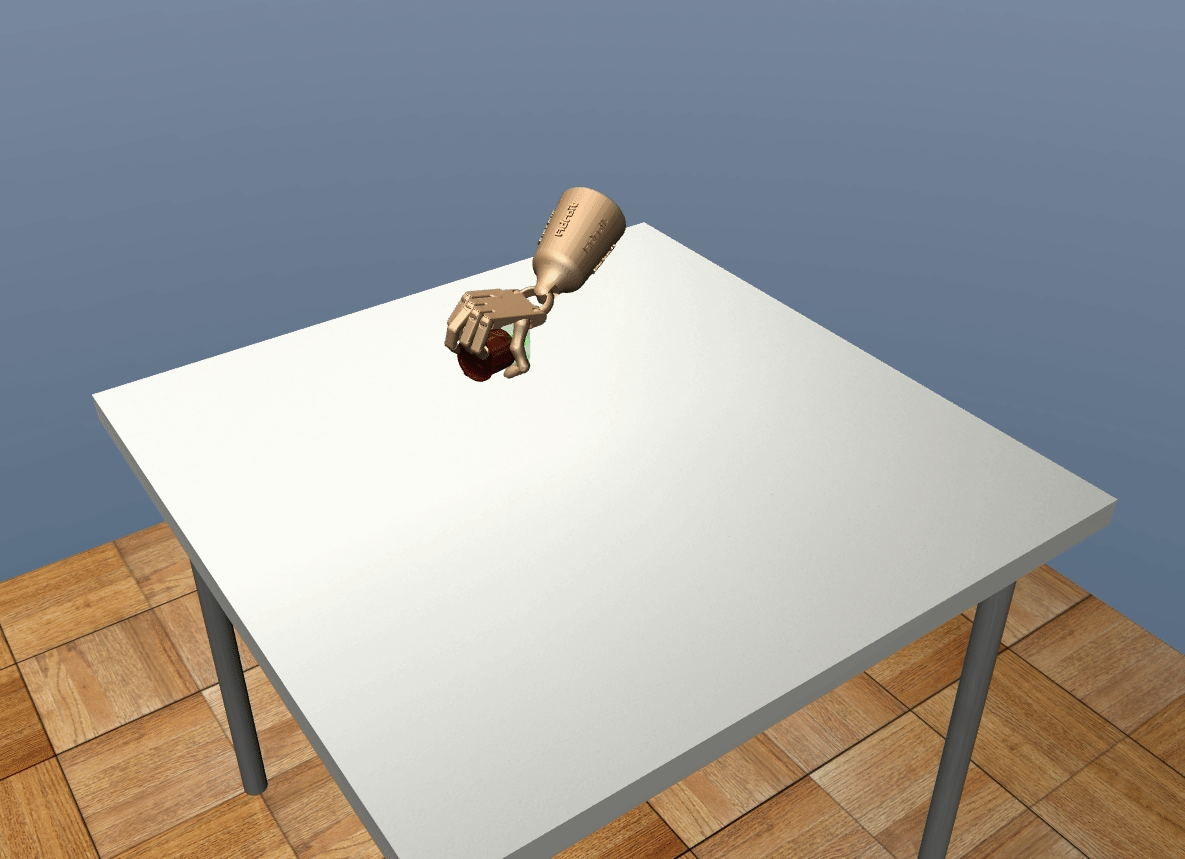
\includegraphics[width=\textwidth]{chapters/3-in-hand-manipulation/fig/frame_44.png}
		\caption{The placing phase, where the mug is placed onto the silhouette.}
		\label{fig:ai-frame-3}
	\end{subfigure}
		\caption{The \gls{pnp} phases executed by the trained \gls{dapg} in MuJoCo}
		\label{fig:ai-frames}
\end{figure}

To compare the trained algorithm to the one provided by the authors, it is of interest to test if the reward distributions resulting from experiments come from the same underlying distribution. To determine this a \gls{anova} test is applied, which requires the presence of normality and homoscedasticity. The normality of each algorithm's performance is tested using normal plots as shown in~\figref{fig:sampled-data-points-vs-normally-distributed-points-authors}. Based on these plots, normality is assumed.

\begin{figure}[!h]
	\centering
	\begin{subfigure}[b]{0.48\textwidth}
		\centering
		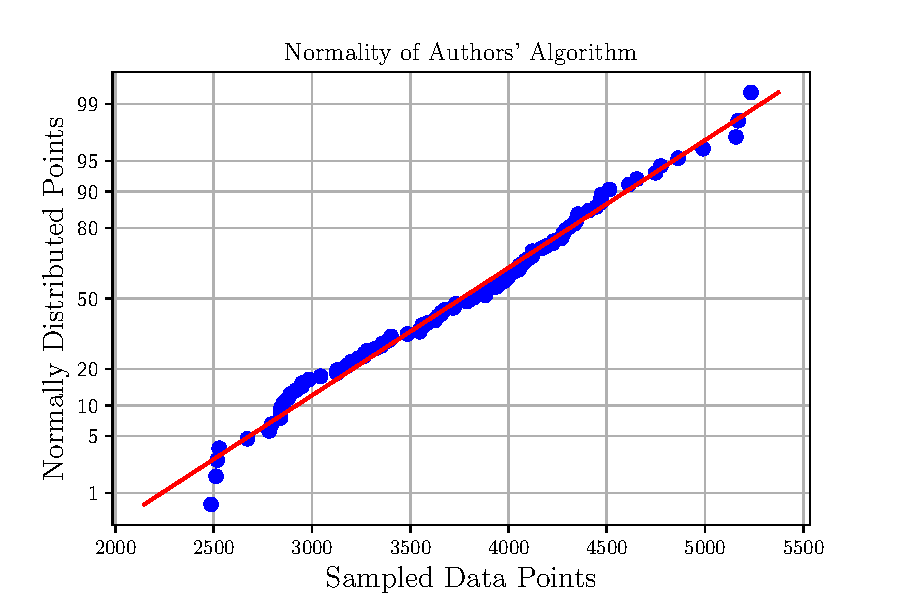
\includegraphics[width=\textwidth]{chapters/3-in-hand-manipulation/fig/sampled-data-points-vs-normally-distributed-points-authors.pdf}
		\caption{Normal plot, showing the extent to which the authors \gls{dapg} algorithm gets rewards that are normally distributed. }
		\label{fig:sampled-data-points-vs-normally-distributed-points-authors}
	\end{subfigure}
	\hfill
	\begin{subfigure}[b]{0.48\textwidth}
		\centering
		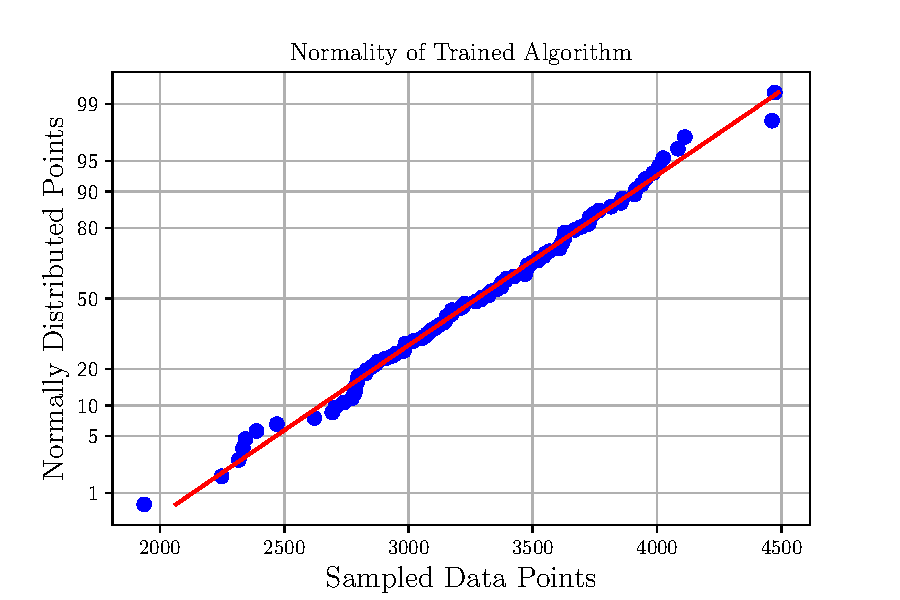
\includegraphics[width=\textwidth]{chapters/3-in-hand-manipulation/fig/sampled-data-points-vs-normally-distributed-points-trained.pdf}
		\caption{Normal plot, showing the extent to which the trained \gls{dapg} algorithm gets rewards that are normally distributed.}
		\label{fig:sampled-data-points-vs-normally-distributed-points-trained}
	\end{subfigure}
	\caption{Normal plots showing the extent to which the performance of the \gls{dapg} algorithms tested in this chapter is normally distributed.}
	\label{fig:sampled-data-points-vs-normally-distributed-points-trained-authors}
\end{figure}

When testing for homoscedasticity the Bartlett test is applied, resulting in the p-value \mvar{p_{bart}\approx 0.0044}. Due to the common threshold for rejecting homoscedasticity being \num{0.05}, which here is considered sufficiently close to \num{0.0044} to attempt a One-Way \gls{anova} test. \medskip

The One-Way \gls{anova} resulted in a p-value of \mvar{p_{\text{ANOVA}}\approx 1.13\cdot 10^{-8}}. \medskip

\newpage

\section{Discussion \& Conclusion}

% This chapter has shown that the \gls{dapg} successfully learn from demonstration and can perform the dexterous manipulation task of relocation. The results from the trained algorithm appear normally distributed but do not strictly fulfill homoscedasticity. Further investigation showed a statistically significant difference between the two underlying distributions, indicating a better performance from the agent trained by the authors.

The findings of this chapter provide strong evidence that the \gls{dapg} algorithm successfully learns from demonstrations and demonstrates its capability to perform the dexterous manipulation task of relocation. The trained algorithm exhibits promising results, with outcomes that follow a distribution resembling a normal distribution.\medskip

However, upon closer analysis, it becomes apparent that the distribution of the algorithm's performance does not strictly adhere to the assumption of homoscedasticity. Homoscedasticity assumes that the variances of the performance values are equal across the distribution. In this case, the observed departure from homoscedasticity suggests the presence of variability or heterogeneity in the algorithm's performance across different relocation tasks. Even so, a One-Way \gls{anova} test was performed which concluded that the reward probability distributions showed statistically significant evidence for having different means. Due to \mvar{\mu_{authors} > \mu_{trained}}, it can be concluded that the authors-trained method performed statistically significantly better than the one trained in this project.  \medskip

As both agents were trained using the same setup but with different seeds, the result would indicate the randomization being the cause of this difference. \medskip
% To gain further insights, additional investigation was conducted to compare the underlying distributions. The results of this investigation revealed a statistically significant difference between the distributions associated with the agent trained by the authors and the alternative distributions. This significant difference implies that the agent trained by the authors outperforms the alternatives in terms of its ability to successfully accomplish the relocation task.\medskip

In summary, the chapter highlights the successful learning capabilities of the \gls{dapg} algorithm from demonstrations, specifically in the context of the dexterous manipulation task of relocation. The outcomes generated by the trained algorithm exhibit a distribution that resembles a normal distribution, although it deviates from strict homoscedasticity. By conducting further analysis and comparing underlying distributions, it was determined that the agent trained by the authors performs statistically significantly better than the alternative approaches.